\subsection{Outils}

Dans le cadre de ce projet, nous avons mis en place diverses méthodes et outils de travail en groupe. Nous avons par exemple utilisé des outils de travail collaboratif pour partager nos ressources et mettre notre travail en commun :
\begin{itemize}
        \item Git : outil de versionnage pour partager le code source de notre application ;
        \item Google Drive : système de stockage et synchronisation de fichiers pour tous les autres documents de notre projet.
\end{itemize}

\subsection{Organisation}

Nous nous sommes régulièrement réunis avec notre encadrant pour discuter de l’avancement du projet ainsi que des futures fonctionnalités à implémenter. Nous avons également effectué des réunions sans notre encadrant pour séparer notre projet en plusieurs tâches et pouvoir répartir le travail. Nous avons ainsi choisi des tâches indépendantes les unes des autres pour que chacun puisse travailler dessus en même temps.

Dans le but de nous assurer de l'avancement de notre projet, nous avons fixé des dates pour plusieurs versions intermédiaires de notre logiciel. Cependant, à cause du retard accumulé, une seule version intermédiaire a pu être produite.

Notre encadrant a suggérée que chaque membre du groupe relève ses temps de travail pour qu'à la fin du projet, il soit possible d'identifier les tâches qui nous ont pris le plus de temps. La synthèses des resultats donne le diagramme de la figure \ref{05-1-work_repartition_chart}.

\begin{figure}
  \begin{center}
  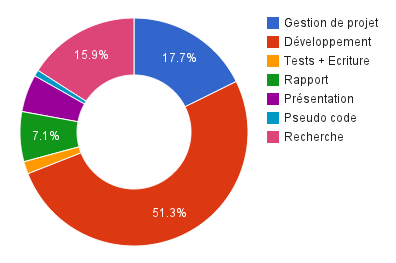
\includegraphics[scale=1]{res/05-1-work_repartition_chart.png}
  \caption{Diagramme de répartition du travail}
  \label{05-1-work_repartition_chart}
  \end{center}
\end{figure}

On remarque que la partie dominante est le développement, car il y avait beaucoup à faire en partant de zéro, contrairement à l'écriture du pseudo-code des algorithmes qui n'a pas été très long. Le développement ne constitue cependant que 50\% du temps, le reste étant principalement consacré à la partie recherche (notamment en probabilités), à la gestion de projet et à la rédaction du rapport et de la présentation.
Nous n'avons malheureusement pas eu le temps d'écrire des tests complets pour notre application, car le développement de son coeur nous a pris trop de temps.


